\documentclass[10pt, compress]{beamer}

\usetheme{m}
\usepackage{amssymb}
\usepackage{graphicx}
\usepackage{booktabs}
\usepackage[scale=2]{ccicons}
\usepackage{minted}
\usemintedstyle{perldoc}

\usepgfplotslibrary{dateplot}

\usemintedstyle{trac}

\usepackage{datetime}
\newdate{date}{03}{08}{2015}

\usepackage{verbatim}
\usepackage{tikz}
%\usetikzlibrary{shapes.geometric, arrows}
\usetikzlibrary{shapes,arrows,shadows}
\tikzstyle{startstop} = [rectangle, rounded corners, minimum width=3cm, minimum height=1cm,text centered, draw=black, fill=red!30]
\tikzstyle{io} = [ellipse, minimum width=3cm, minimum height=1cm, text centered, draw=black, fill=blue!30,
,inner sep=0.5ex,font=\sffamily]
\tikzstyle{arrow} = [thick,->,>=stealth]
\def\checkmark{\tikz\fill[scale=0.4](0,.35) -- (.25,0) -- (1,.7) -- (.25,.15) -- cycle;}
\newcounter{cnt}
\setcounter{cnt}{0}

\newcommand{\distpic}[3]{
    % First draw the upper distribution.
    % Shade the critical region:
    \fill[red!30] (0.658,0)  -- plot[id=f3,domain=0.658:3,samples=50]
        function {exp(-x*x*0.5/0.16)} -- (3,0) -- cycle;

    % Draw the normal distribution curve
    \draw[blue!50!black,smooth,thick] plot[id=f1,domain=-2:3,samples=50]
    function {exp(-x*x*0.5/0.16)};
    % Draw the x-axis
    \draw[->,black] (-2.2,0) -- (3.2,0);
    % Put some ticks and tick labels in:
    \foreach \x in {-2,-1,0,1,2,3}
    \draw (\x,0) -- (\x,-0.1) node[below] {$\x$};
    % Put in a label for the critical region boundary:
    \draw[red!50!black,thick] (0.658,0) node[below,yshift=-0.5cm] {0.658}
    -- (0.658,0.85);

    % Put in labels for accepting or rejecting the null hypothesis with
    % the corresponding regions:
    \draw[red!50!black,thick,->] (0.688,0.7) -- (1.3,0.7)
        node[anchor=south] {Reject  $H_0$};
    \draw[red!50!black,thick,->] (0.628,0.7) -- (-1,0.7)
        node[anchor=south]{\parbox{1.5cm}{\raggedright Fail to reject $H_0$}};

    % Add a label to the upper picture, when the null is true
    \draw (-3,1) node[above,draw,fill=green!30] {$H_0$ is true:};

    % Label the critical region with an alpha level:
    \draw[<-,thick] (0.75,0.05) -- (1.6,0.2) node[right,yshift=0.3cm]
    {\begin{tabular}{l} $\alpha=0.05$ \\ (Type I error rate) \end{tabular}};


    % Add a label showing the effect size between the two plots:
    \draw[very thin] (0,-1) -- (0,-0.5);
    \draw[<->,thick] (0,-1) node[left] {Effect size:  #1} -- (#1,-1);
    \draw[thick] (0,-.9) -- (0,-1.1);

    \draw[very thin] (#1,-1) -- (#1,-1.7);
    \draw[thick] (#1,-.9) -- (#1,-1.1);

    % Now draw the lower distribution showing the effect size:
    \begin{scope}[yshift=-3cm]
    % Shade the "reject H0" region red
    \fill[red!30] (0.658,0)  -- plot[id=f3\thecnt,domain=0.658:3,samples=50]
        function {exp(-(x-#1)*(x-#1)*0.5/0.16)} --
        (3,0) -- cycle;
        % Shade the "accept H0" region blue
    \fill[blue!30] (-2,0) -- plot[id=f4\thecnt,domain=-2:0.658,samples=50]
        function {exp(-(x-#1)*(x-#1)*0.5/0.16)} --
        (0.658,0) -- cycle;

        % Draw the shifted normal distribution:
    \draw[blue!50!black,smooth,thick] plot[id=f1\thecnt,domain=-2:3,samples=50]
            function {exp(-(x-#1)*(x-#1)*0.5/0.16)};

        % Draw the x-axis and put in some ticks and tick labels
    \draw[->,black] (-2.2,0) -- (3.2,0);
    \foreach \x in {-2,-1,0,1,2,3}
            \draw (\x,0) -- (\x,-0.1) node[below] {$\x$};

        % Draw and label the critical region boundary
    \draw[red!50!black,very thick] (0.658,0) node[below,yshift=-0.5cm] {0.658}
        -- (0.658,1.0);
    \draw[red!50!black,very thick,->] (0.688,0.7) -- (2.7,0.7)
        node[anchor=south west] {Reject  $H_0$};
    \draw[red!50!black,very thick,->] (0.628,0.7) -- (-0.5,0.7)
        node[anchor=south]{\parbox{1.5cm}{\raggedright Fail to reject $H_0$}};

    % Add a label to the lower picture, when the alternative hypothesis is true:
    \draw (-3,1) node[above,draw,fill=green!30] {$H_a$ is true:};

        % Add labels showing the statistical power and the Type II error rate:
    \draw[<-,thick] (1.5,0.1) -- (3,0.2) node[anchor=south west]
        {Power = \large #2};
    \draw[<-,thick] (0.4,0.1) -- (-1,0.2) node[left,yshift=0.3cm]
        {\begin{tabular}{l}
        $\beta$ = {\large #3} \\ (Type II error rate) \end{tabular}};
    \end{scope}
}


\title{Advanced Quantitative Methods Clinic}
\subtitle{Master’s in Sustainability Leadership,\\
Cambridge Institute for Sustainability Leadership}
\date{\displaydate{date}}
\author{Sreekumar Thaithara Balan}
\institute{Department of Physics and Astronomy,\\
University College London\\
sbalan@star.ucl.ac.uk,
@sreekumar\_balan}

\begin{document}

\maketitle

%
\section{Outline}

\begin{frame}
    \frametitle{Outline}
    \begin{itemize}
        \item Software for data analysis ($\sim$15mins)
        \item Data visualisation ($\sim$20mins)
        \item Descriptive statistics ($\sim$20mins)
        \item Inferential statistics ($\sim$20mins)
        \item Regression ($\sim$20mins)
        \item Discussion ($\sim$10mins)
    \end{itemize}
\end{frame}

\section{Software for data analysis}

\begin{frame}
    \frametitle{Repository}
    Supplementary materials can found at \\
    \url{https://github.com/tbs1980/CISLQuantWorkshop}
\end{frame}

\begin{frame}[fragile]
    \frametitle{Software for data analysis}
    A large list can be found in \href{https://en.wikipedia.org/wiki/List_of_statistical_packages}{\texttt{Wikipedia}}.
    Some widely used ones are below.
    \begin{itemize}
        \item \texttt{Python}, \url{https://www.python.org/} %{\texttt{Python}}
        \item \texttt{R}, \url{https://cran.r-project.org/}%{\texttt{R}}
        \item \texttt{Excel}, \url{https://products.office.com/en-us/excel}%{\texttt{Excel}}
        \item \texttt{SPSS}, \url{http://www-01.ibm.com/software/analytics/spss/}
    \end{itemize}
    I will demonstrate the examples using \texttt{Python}. If you have no prior
    experience, no problem, there will be plenty of help.
\end{frame}

\begin{frame}[fragile]
    \frametitle{Software set-up}
    We need at least one of the statistical software mentioned in the
    previous slide. Please follow the instructions below
    \begin{itemize}
        \item \url{http://docs.continuum.io/anaconda/install}%{\texttt{Python}}
        \item \url{https://cran.r-project.org/}%{\texttt{R}}
        \item \url{https://products.office.com/en-us/excel}%{\texttt{Excel}}
        \item \url{http://www-01.ibm.com/software/analytics/spss/}
    \end{itemize}
    \smallskip
    %\alert{Has everyone installed one of the above?}
\end{frame}

\section{Data visualisation}

\begin{frame}
    \frametitle{Data visualisation}
    \begin{columns}
        \column{0.5\textwidth}
        \begin{block}{examples}
            \begin{itemize}
                \item{bar-charts}
                \item{histograms}
                \item{scatter-plots}
                \item{error-bars}
                \item{pie-charts}
                \item{many more!}
            \end{itemize}
        \end{block}
        %
        \column{0.5\textwidth}
        \begin{block}{}
            %\alert{\huge A picture is worth a thousand words}
            \begin{figure}
                \begin{center}
                    \includegraphics[scale=0.2]{img/121236_NewPieCharts720.png}
                    %http://map.gsfc.nasa.gov/universe/uni_matter.html
                \end{center}
                %\footnote{\tiny{\url{http://map.gsfc.nasa.gov/universe/uni_matter.html}}}
            \end{figure}
        \end{block}
        %
    \end{columns}
    %Figure from \footnote{\tiny{\url{http://map.gsfc.nasa.gov/universe/uni_matter.html}}}
\end{frame}

\begin{frame}
    \frametitle{Data visualisation: Examples}
    \begin{itemize}
        \item We have several examples in the repository.
        \item Please follow the instructions in \url{https://github.com/tbs1980/CISLQuantWorkshop/tree/master/AdvancedQuantitativeMethodsClinic}.
        \item \alert{clustering}
        \item \alert{outliers}
        \item \alert{normalisation}
        %\item We have 15 mins for this session.
        %\item Get your hands dirty!
    \end{itemize}
\end{frame}

\section{Descriptive statistics}

\begin{frame}
    \frametitle{Descriptive statistics}
    \begin{itemize}
        \item Definitions
        \item Frequency distributions
        \item Central tendency and variability
    \end{itemize}
\end{frame}

\begin{frame}
    \frametitle{Definitions}
    \begin{columns}
        \column{0.5\textwidth}
        \begin{block}{Glossary}
            \begin{itemize}
                \item Population
                \item Samples
                \item Variable
                \item Data
                \item Parameter
                \item Statistic
            \end{itemize}
        \end{block}
        %
        \column{0.5\textwidth}
        \begin{block}{}
            \begin{figure}
                \begin{center}
                    \includegraphics[scale=0.7]{img/as1-10-popvsam.png}
                    %http://ihsmath11.wikispaces.com/AS1.10+Population+vSample
                \end{center}
            \end{figure}
        \end{block}
    \end{columns}
\end{frame}

%
% TODO MORE SLIDES ON THE DEFINITIONS
%

\begin{frame}
    \frametitle{Freqency distributions}
    \begin{columns}
        \column{0.5\textwidth}
        \begin{block}{Defined by}
            \begin{itemize}
                \item Size
                \item Range
                \item Bins-size
                \item Normalisation
            \end{itemize}
        \end{block}
        %
        \column{0.5\textwidth}
        \begin{block}{}
            \begin{figure}
                \begin{center}
                    \includegraphics[scale=0.3]{img/hist_new_stacked.png}
                    %http://pandas.pydata.org/pandas-docs/stable/visualization.html
                \end{center}
            \end{figure}
        \end{block}
    \end{columns}
\end{frame}

\begin{frame}
    \frametitle{Central tendency}
    \begin{columns}
        \column{0.5\textwidth}
        \begin{block}{How to characterise a distribution?}
            \begin{itemize}
                \item \alert{What is a measure of central tendency?}
                \item Mean, median and mode
            \end{itemize}
            \smallskip
            The mean $\mu$ of samples $\{x_1,x_2,\cdots,x_n\}$ can be computed
            as
            \begin{equation}
                \mu = \frac{\sum_i x_i}{n}
            \end{equation}
        \end{block}
        %
        \column{0.5\textwidth}
        \begin{block}{}
            \begin{figure}
                \begin{center}
                    \includegraphics[scale=0.5]{img/central_tendancy.jpg}
                    %http://flowjo.typepad.com/the_daily_dongle/science/
                \end{center}
            \end{figure}
        \end{block}
    \end{columns}
\end{frame}

\begin{frame}
    \frametitle{Variability}
    \begin{columns}
        \column{0.5\textwidth}
        \begin{block}{How to measure variations?}
            \begin{itemize}
                \item \alert{Are you a good shooter?}
                \item Variance and standard deviation
                \item Population and samples
            \end{itemize}
            \smallskip
            The (biased) samples variance is defined as
            \begin{equation}
                \sigma^2 = \frac{\sum_i (x_i - \mu)^2}{n}
            \end{equation}
            We also define sums of squares $SS$ as
            \begin{equation}
                SS = \sum x^2
            \end{equation}
        \end{block}
        %
        \column{0.5\textwidth}
        \begin{block}{}
            \begin{figure}
                \begin{center}
                    \includegraphics[scale=0.4]{img/std_dvn.png}
                    %http://www.itrcweb.org/ism-1/4_3_1_3_Relative_standard_deviation_of_replicate_samples.html
                \end{center}
            \end{figure}
        \end{block}
    \end{columns}
\end{frame}

\begin{frame}
    \frametitle{Examples/Discussion}
    \begin{itemize}
        \item \alert{How do we characterise skewed distributions?}
        \item \alert{Concept of moments}
        \item \alert{Distributions outside law of large numbers}
        \item Examples can be found at \url{https://github.com/tbs1980/CISLQuantWorkshop/tree/master/AdvancedQuantitativeMethodsClinic/examples}
        \item Use the rest of the time for examples/discussion.
    \end{itemize}
\end{frame}

\section{Inferential statistics}

\begin{frame}
    \frametitle{Inferential statistics}
    \begin{itemize}
        \item Probability
        \item The Normal distribution
        \item Sample means and their distribution
        \item Introduction to hypothesis testing
    \end{itemize}
\end{frame}

\begin{frame}
    \frametitle{Probability}
    \begin{columns}
        \column{0.5\textwidth}
        \begin{block}{Frequency or degree of belief?}
            \begin{itemize}
                \item Frequency
                \item Desired outcome
                \item Random sample
            \end{itemize}
        \end{block}
        %
        \column{0.5\textwidth}
        \begin{block}{}
            \begin{figure}
                \begin{center}
                    \includegraphics[scale=0.2]{img/GRE_Probability.png}
                    %http://www.brightlinkprep.com/wp-content/uploads/2013/04/GRE_Probability.png
                \end{center}
            \end{figure}
        \end{block}
    \end{columns}
\end{frame}


\begin{frame}
    \frametitle{Role of Probability}
    \begin{columns}
        \column{0.5\textwidth}
        \begin{itemize}
            \item What kind of samples are likely to obtained from the population?
            \item What can we say about the population given a sample?
        \end{itemize}
        \column{0.5\textwidth}
        \begin{figure}
            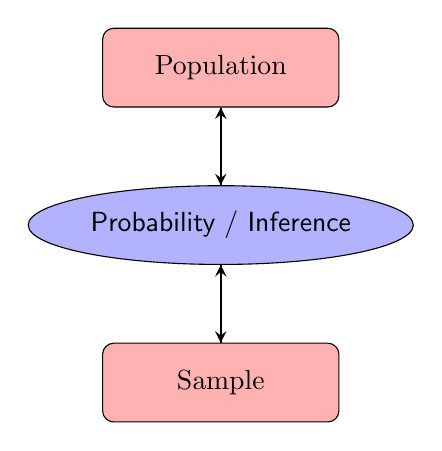
\begin{tikzpicture}[node distance=2cm]
                \node (pop) [startstop] {Population};
                \node (prob) [io,below of= pop] {Probability / Inference};
                \node (samp) [startstop,below of= prob] {Sample};
                \draw [arrow] (pop) -- (prob);
                \draw [arrow] (prob) -- (samp);
                \draw [arrow] (samp) -- (prob);
                \draw [arrow] (prob) -- (pop);
            \end{tikzpicture}
        \end{figure}
    \end{columns}
\end{frame}


\begin{frame}
    \frametitle{The Normal distribution}
    \begin{columns}
        \column{0.5\textwidth}
        \begin{block}{Characteristics}
            \begin{itemize}
                \item Mean $\mu$
                \item Standard deviation $\sigma$
                \item \alert{Why is it important?}
                \item Distribution of sample means
            \end{itemize}
            \smallskip
            \begin{equation}
                \Pr(x|\mu,\sigma)  = \frac{1}{\sigma\sqrt{2\pi}}
                    \exp\left(-\frac{1}{2}\frac{(x-\mu)^2}{\sigma^2}\right)
            \end{equation}
        \end{block}
        %
        \column{0.5\textwidth}
        \begin{block}{}
            \begin{figure}
                \begin{center}
                    \includegraphics[scale=0.4]{img/normal-curve.png}
                    %http://www.had2know.com/academics/normal-distribution-probability-calculator.html
                \end{center}
            \end{figure}
        \end{block}
    \end{columns}
\end{frame}

\begin{frame}
    \frametitle{Sample means and their distribution}
    \begin{columns}
        \column{0.5\textwidth}
        \begin{block}{Characteristics}
            \begin{itemize}

                \item Sampling error
                \item Distribution of sample means
                \item Expected value
                \item Standard error
                \item Law of large numbers
            \end{itemize}
            The standard error is defined as
            \begin{equation}
                \sigma_M = \frac{\sigma}{n}
            \end{equation}
        \end{block}
        %
        \column{0.5\textwidth}
        \begin{block}{}
            \begin{figure}
                \begin{center}
                    \includegraphics[scale=0.3]{img/14_diag_b.png}
                    %https://epilab.ich.ucl.ac.uk/coursematerial/statistics/inference/standard_error.html
                \end{center}
            \end{figure}
        \end{block}
    \end{columns}
\end{frame}

\begin{frame}
    \frametitle{Hypothesis testing}
    \begin{columns}
        \column{0.5\textwidth}
        \begin{block}{Baic idea}
            \begin{itemize}
                \item Known versus unknown
                \item Null versus alternative hypothesis
                \item Decision criteria
                \item Level of significance
                \item Critical region
                \item Uncertainty and errors
                \item Statistical significance
            \end{itemize}
        \end{block}
        %
        \column{0.5\textwidth}
        \begin{block}{}
            \begin{figure}
                \begin{center}
                    \includegraphics[scale=0.3]{img/IQ_Hypoth.png}
                    %http://simon.cs.vt.edu/SoSci/converted/Hypoth_I/
                \end{center}
            \end{figure}
        \end{block}
    \end{columns}
\end{frame}

\begin{frame}
    \frametitle{Logic behind hypothesis testing}
    \begin{columns}
        \column{0.5\textwidth}
        \begin{block}{Questions}
            \begin{itemize}
                \item Can we observe meaningful patterns in the data
                \item Are the findings statistically significant?
                \item Does the model adequately describe the data?
                \item Is there evidence for an alternative hypothesis?
            \end{itemize}
        \end{block}
        %
        \column{0.5\textwidth}
        \begin{block}{}
            \begin{figure}
                \scalebox{0.7}
                {
                    \begin{tikzpicture}
                        \def \n {2}
                        \def \radius {3cm}
                        \def \margin {6}
                        \def \s {1}
                        \node[draw, circle] at ({360/\n * (\s - 1)}:\radius) {Model};
                            \draw[->, >=latex] ({360/\n * (\s - 1)+\margin}:\radius)
                                arc ({360/\n * (\s - 1)+\margin}:{360/\n * (\s)-\margin}:\radius);
                        \def \s {2}
                        \node[draw, circle] at ({360/\n * (\s - 1)}:\radius) {Data};
                            \draw[->, >=latex] ({360/\n * (\s - 1)+\margin}:\radius)
                                arc ({360/\n * (\s - 1)+\margin}:{360/\n * (\s)-\margin}:\radius);
                    \end{tikzpicture}
                }
            \end{figure}
        \end{block}
    \end{columns}
\end{frame}

\begin{frame}
    \frametitle{hypothesis testing by comparing distributions}
    \begin{columns}
        \column{0.5\textwidth}
        \begin{block}{}
            \begin{itemize}
                \item Known characteristics of a population
                \item Selected sample for research
                \item Characteristics of the sample after experiment
                \item How do they compare?
            \end{itemize}
            \smallskip
            We deifne  $z$-score as
            \begin{equation}
                z = \frac{M-\mu}{\sigma_M}
            \end{equation}
        \end{block}
        %
        \column{0.5\textwidth}
        \begin{block}{}
            \begin{figure}
                \scalebox{0.7}
                {
                    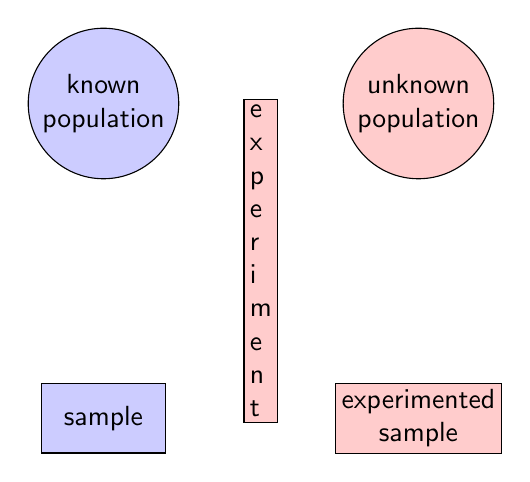
\begin{tikzpicture}
                        \node[draw, fill=red!20, rectangle, align=left,
                            inner sep=0.5ex, font=\sffamily]
                            at (0,0) { e \\ x \\ p \\ e \\ r \\ i \\ m \\ e \\ n \\ t };
                        \node[draw, fill=red!20,circle,align=center,inner sep=0.5ex,font=\sffamily]
                            at (2,2) {unknown \\ population};
                        \node[draw,fill=red!20,rectangle,align=center,inner sep=0.5ex,font=\sffamily]
                            at (2,-2) {experimented \\ sample};
                        \node[draw, fill=blue!20,circle,,align=center,inner sep=0.5ex,font=\sffamily]
                            at (-2,2) {known \\ population};
                        \node[draw,fill=blue!20,rectangle,align=center,
                            minimum height=2.5em,minimum width=4.5em,inner sep=0.5ex,font=\sffamily]
                            at (-2,-2) {sample};
                    \end{tikzpicture}
                }
            \end{figure}
        \end{block}
    \end{columns}
\end{frame}

\begin{frame}
    \frametitle{Comparing changes in $\mu$}
    \begin{figure}
        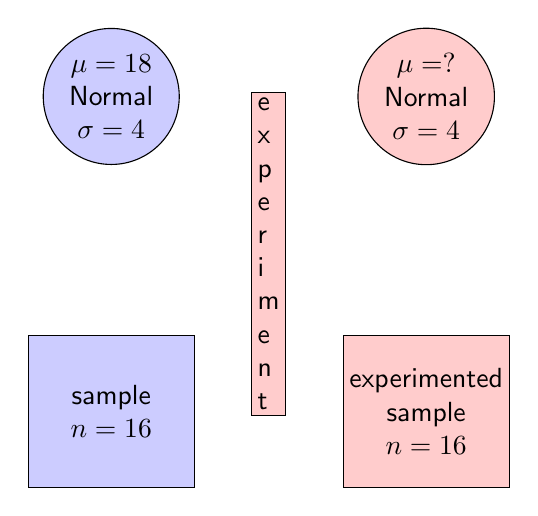
\begin{tikzpicture}
            \node[draw, fill=red!20, rectangle, align=left,
                inner sep=0.5ex, font=\sffamily]
                at (0,0) { e \\ x \\ p \\ e \\ r \\ i \\ m \\ e \\ n \\ t };
            \node[draw, fill=red!20,circle,align=center,inner sep=0.5ex,font=\sffamily]
                at (2,2) {$\mu =?$ \\ Normal \\ $\sigma=4$};
            \node[draw,fill=red!20,rectangle,align=center,
                minimum height=5.5em,minimum width=6em,inner sep=0.5ex,font=\sffamily]
                at (2,-2) {experimented \\ sample \\ $n=16$};
            \node[draw, fill=blue!20,circle,,align=center,inner sep=0.5ex,font=\sffamily]
                at (-2,2) {$\mu =18$ \\ Normal \\ $\sigma=4$};
            \node[draw,fill=blue!20,rectangle,align=center,
                minimum height=5.5em,minimum width=6em,inner sep=0.5ex,font=\sffamily]
                at (-2,-2) {sample \\ $n=16$};
        \end{tikzpicture}
    \end{figure}
\end{frame}


\begin{frame}
    \frametitle{Comparing changes in $\mu$: statistical odds}
    \begin{figure}
        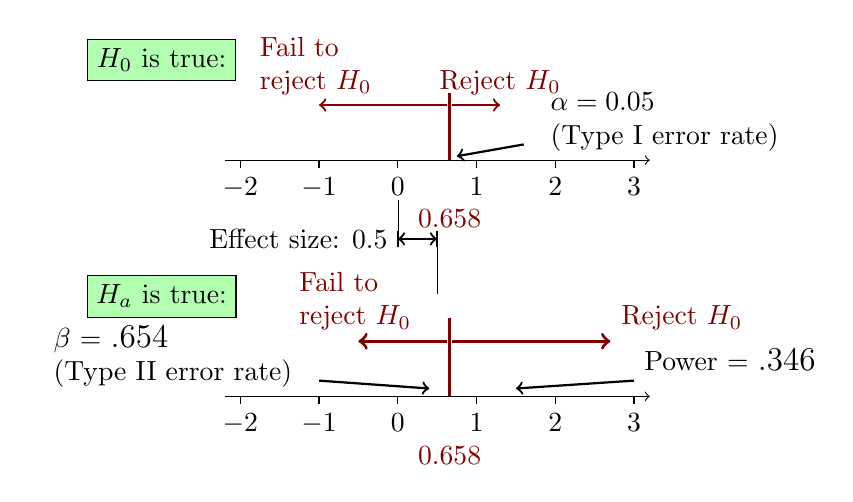
\begin{tikzpicture}
            \distpic{0.5}{.346}{.654}
        \end{tikzpicture}
    \end{figure}
\end{frame}

\begin{frame}
    \frametitle{Examples/Discussion}
    \begin{itemize}
        \item \alert{What if the $H_0$ is false?}
        \item \alert{How accurate is the $\sigma$ invariance assumption?}
        \item \alert{How will we choose the level of significance?}
        \item Examples can be found at \url{https://github.com/tbs1980/CISLQuantWorkshop/tree/master/AdvancedQuantitativeMethodsClinic/examples}
        \item Use the rest of the time for examples/discussion.
    \end{itemize}
\end{frame}

\section{Inferences about Population Means}

\begin{frame}
    \frametitle{Inferences about Population Means}
    \begin{itemize}
        \item $t$-statistic
        \item ANalysis Of VAriacne (ANOVA)
    \end{itemize}
\end{frame}

\begin{frame}
    \frametitle{Introduction to $t$-statistic}
    \begin{columns}
        \column{0.5\textwidth}
        \begin{block}{Motivation}
            \begin{itemize}
                \item Population $\sigma$ unknown
                \item How can we compare means?
                \item Estimated standard error, $s_M$
                \item Degrees of freedom, $df$
            \end{itemize}
            \smallskip
            We define the $t$-statistics as
            \begin{equation}
                t = \frac{M-\mu}{s_M}
            \end{equation}
            and percentage of variance as
            \begin{equation}
                r^2 = \frac{t^2}{t^2+df}
            \end{equation}
        \end{block}
        \column{0.5\textwidth}
        \begin{block}{}
            \begin{figure}
                \begin{center}
                    \includegraphics[scale=0.17]{img/2289604_orig.png}
                    % http://www.stats4stem.org/uploads/1/7/6/7/1767713/2289604_orig.png
                \end{center}
            \end{figure}
        \end{block}

    \end{columns}
\end{frame}

\begin{frame}
    \frametitle{Comparing two sets of data}
    \begin{columns}
        \column{0.5\textwidth}
        \begin{block}{How do we compare?}
            \begin{itemize}
                \item Are there differences between population means?
            \end{itemize}
        \end{block}
        {\small
            \begin{align}
                t & = \frac{(M_1-M_2)-(\mu_1-\mu_2)}{s_{(M_1-M_2)}} \\
                s_{(M_1-M_2)} &= \sqrt{\frac{s_p^2}{n_1}+\frac{s_p^2}{n_2}} \\
                s_p & = \frac{SS_1 + SS_2}{df} \\
                df & = df_1 + df_2
            \end{align}
        }
        \column{0.5\textwidth}
        \begin{block}{}
            \begin{figure}
                \scalebox{0.7}
                {
                    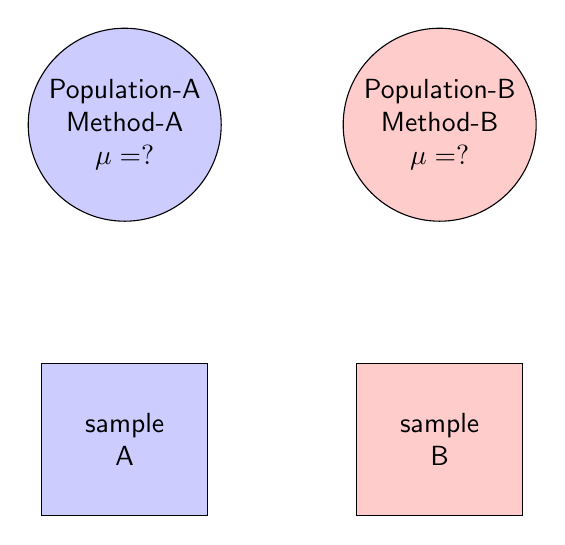
\begin{tikzpicture}
                        \node[draw, fill=red!20,circle,align=center,inner sep=0.5ex,font=\sffamily]
                            at (2,2) {Population-B \\ Method-B \\ $\mu =?$};
                        \node[draw,fill=red!20,rectangle,align=center,
                            minimum height=5.5em,minimum width=6em,inner sep=0.5ex,font=\sffamily]
                            at (2,-2) {sample \\ B};
                        \node[draw, fill=blue!20,circle,,align=center,inner sep=0.5ex,font=\sffamily]
                            at (-2,2) {Population-A \\ Method-A \\ $\mu =?$};
                        \node[draw,fill=blue!20,rectangle,align=center,
                            minimum height=5.5em,minimum width=6em,inner sep=0.5ex,font=\sffamily]
                            at (-2,-2) {sample \\ A};
                    \end{tikzpicture}
                }
            \end{figure}
        \end{block}
    \end{columns}
\end{frame}

\begin{frame}
    \frametitle{ANlysis Of VAriacne (ANOVA)}
    \begin{columns}
        \column{0.5\textwidth}
        \begin{block}{}
            \begin{itemize}
                \item Different samples for different experiments
                \item Are the results statistically different?
                \item How to differentiate between random and systematic variations?
                \item $H_0:\mu_1 = \mu_2 = \mu_3$
                \item $H_1:$ at least one mean differences
            \end{itemize}
        \end{block}
        \column{0.5\textwidth}
        \begin{block}{}
            \begin{figure}
                \scalebox{0.6}
                {
                    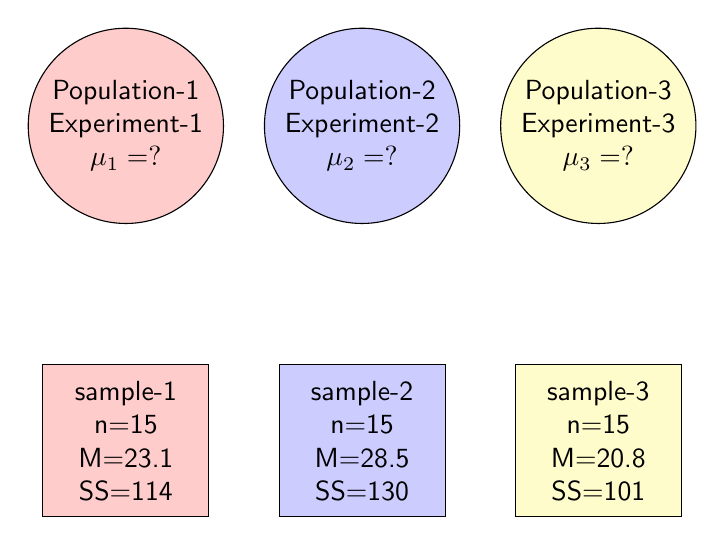
\begin{tikzpicture}
                        \node[draw, fill=red!20,circle,align=center,inner sep=0.5ex,font=\sffamily]
                            at (-3,2) {Population-1 \\ Experiment-1 \\ $\mu_1 =?$};
                        \node[draw, fill=blue!20,circle,align=center,inner sep=0.5ex,font=\sffamily]
                            at (0,2) {Population-2 \\ Experiment-2 \\ $\mu_2 =?$};
                        \node[draw, fill=yellow!20,circle,align=center,inner sep=0.5ex,font=\sffamily]
                            at (3,2) {Population-3 \\ Experiment-3 \\ $\mu_3 =?$};
                        \node[draw,fill=red!20,rectangle,align=center,minimum height=5.5em,
                            minimum width=6em,inner sep=0.5ex,font=\sffamily]
                            at (-3,-2) {sample-1 \\ n=15 \\ M=23.1 \\ SS=114};
                        \node[draw,fill=blue!20,rectangle,align=center,minimum height=5.5em,
                            minimum width=6em,inner sep=0.5ex,font=\sffamily]
                            at (0,-2) {sample-2 \\ n=15 \\ M=28.5 \\ SS=130};
                        \node[draw,fill=yellow!20,rectangle,align=center,minimum height=5.5em,
                            minimum width=6em,inner sep=0.5ex,font=\sffamily]
                            at (3,-2) {sample-3 \\ n=15 \\ M=20.8 \\ SS=101};
                    \end{tikzpicture}
                }
            \end{figure}
        \end{block}
    \end{columns}
\end{frame}

\begin{frame}
    \frametitle{ANOVA: The fundamental concept}
    \begin{columns}
        \column{0.5\textwidth}
        \begin{block}{Measuring variability}
            Recap: we can write the $t$-statistic as
            \begin{equation}
                \small
                t = \frac{\text{difference between sample means}}{\text{standard error}}
            \end{equation}
            We define $F$-statistic as
            \begin{equation}
                \small
                F = \frac{\text{variance between sample means}}{\text{intrinsic variance}}
            \end{equation}
            \begin{itemize}
                \item systematic effects
                \item random, unsystematic factors
            \end{itemize}
        \end{block}
        \column{0.5\textwidth}
        \begin{block}{}
            \begin{figure}
                \scalebox{0.7}
                {
                    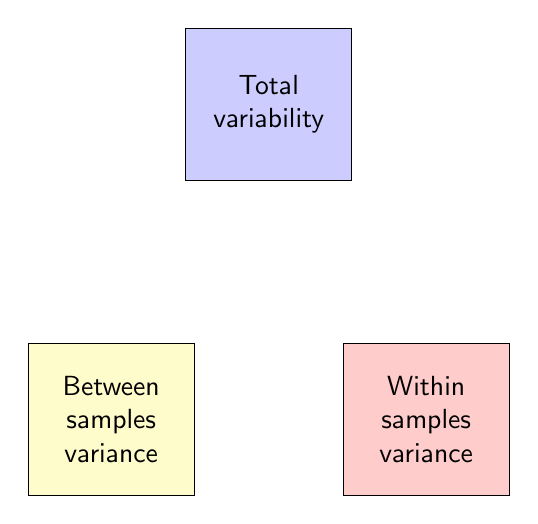
\begin{tikzpicture}
                        \node[draw,fill=blue!20,rectangle,align=center,minimum height=5.5em,
                            minimum width=6em,inner sep=0.5ex,font=\sffamily]
                            at (0,2) {Total \\ variability};
                        \node[draw,fill=yellow!20,rectangle,align=center,minimum height=5.5em,
                            minimum width=6em,inner sep=0.5ex,font=\sffamily]
                            at (-2,-2) {Between\\samples\\variance};
                        \node[draw,fill=red!20,rectangle,align=center,minimum height=5.5em,
                            minimum width=6em,inner sep=0.5ex,font=\sffamily]
                            at (2,-2) {Within\\samples\\variance};
                    \end{tikzpicture}
                }
            \end{figure}
        \end{block}
    \end{columns}
\end{frame}

\begin{frame}
    \frametitle{Computing ANOVA}
    \begin{columns}
        \column{0.5\textwidth}
        \begin{block}{formulae}
            \begin{align}
                SS & = \sum x^2 - \frac{(\sum x)^2}{N} \\
                s^2 & = \frac{SS}{df} \\
                F & = \frac{s^2_{\mathsf{between}}}{s^2_{\mathsf{within}}}
            \end{align}
        \end{block}
        \column{0.5\textwidth}
        \begin{block}{}
            \begin{figure}
                \scalebox{0.7}
                {
                    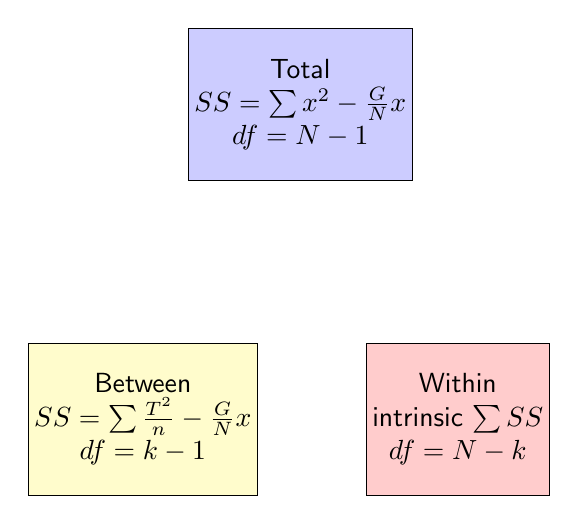
\begin{tikzpicture}
                        \node[draw,fill=blue!20,rectangle,align=center,minimum height=5.5em,
                            minimum width=6em,inner sep=0.5ex,font=\sffamily]
                            at (0,2) {Total \\ $SS = \sum x^2 - \frac{G}{N}x$ \\ $df = N-1$};
                        \node[draw,fill=yellow!20,rectangle,align=center,minimum height=5.5em,
                            minimum width=6em,inner sep=0.5ex,font=\sffamily]
                            at (-2,-2) {Between\\$SS = \sum\frac{T^2}{n} - \frac{G}{N}x$\\$df = k-1$};
                        \node[draw,fill=red!20,rectangle,align=center,minimum height=5.5em,
                            minimum width=6em,inner sep=0.5ex,font=\sffamily]
                            at (2,-2) {Within\\intrinsic $\sum SS$\\$df = N-k$};
                    \end{tikzpicture}
                }
            \end{figure}
        \end{block}
    \end{columns}
\end{frame}

\begin{frame}
    \frametitle{F-statistic}
    \begin{figure}
        \begin{centering}
            \includegraphics[scale=0.7]{img/ftest.png}
        \end{centering}
    \end{figure}
\end{frame}

\begin{frame}
    \frametitle{Examples/Discussion}
    \begin{itemize}
        \item Link to examples \url{https://github.com/tbs1980/CISLQuantWorkshop/tree/master/AdvancedQuantitativeMethodsClinic/examples}
        \item Use the rest of the time for examples/discussion.
    \end{itemize}
\end{frame}

\section{Regression}

\begin{frame}
    \frametitle{Regression}
    \begin{itemize}
        \item Correlation
        \item Parametric-regression
        \item $\chi^2$-test
    \end{itemize}
\end{frame}

\begin{frame}
    \frametitle{Correlation}
    \begin{columns}
        \column{0.5\textwidth}
        \begin{block}{Covariability}
            \begin{itemize}
                \item \alert{linear} relationship between two variables $x$ and $y$
                \item positive and negative
            \end{itemize}
            Pearson correlation is defined as
            \begin{equation}
                \small
                r = \frac{\text{co-variability of X and Y}}{\text{individual variability of X and Y}}
            \end{equation}
            \begin{align}
                SP_{xy} & = \sum xy - \frac{\sum x \sum y}{n} \\
                r &= \frac{S_{xy}}{\sqrt{SS_{xx}SS_{yy}}}
            \end{align}
        \end{block}
        \column{0.5\textwidth}
        \begin{block}{Visualisation}
            \begin{figure}
                \begin{center}
                    \includegraphics[scale=0.2]{img/correlationcoefficient.png}
                    % https://statsmethods.wordpress.com/2013/05/10/pearson-correlation-coefficient-r/
                \end{center}
            \end{figure}
            \begin{itemize}
                \item \alert{outliers}
                \item \alert{correlation and causation}
            \end{itemize}
        \end{block}
    \end{columns}
\end{frame}

\begin{frame}
    \frametitle{Regression}
    \begin{columns}
        \column{0.5\textwidth}
        \begin{block}{Basics}
            \begin{itemize}
                \item Model Vs data
                \item Predicted Vs observed
                \item Parametric Vs non-parametric
                \item Signal and noise
                \item Residuals
                \item $y = f(x) + n$
                \item least-squares
            \end{itemize}
        \end{block}
        \column{0.5\textwidth}
        \begin{block}{}
            \begin{figure}
                \begin{center}
                    \includegraphics[scale=0.2]{img/regression.png}
                    % http://plot1.micw.eu/uploads/Main/regression.png
                \end{center}
            \end{figure}
        \end{block}
    \end{columns}
\end{frame}

\begin{frame}
    \frametitle{Linear model}
    \begin{columns}
        \column{0.5\textwidth}
        \begin{block}{Computation}
            Linear model can be written as
            \begin{equation}
                y = a + bx
            \end{equation}
            $a$ and $b$ can be calculated as
            \begin{align}
                b & = \frac{SS_{yy}}{SS_{xx}} \\
                a & = M_{y} - bM_{x}
            \end{align}
            The standard error is
            \begin{equation}
                err_{std} = \sqrt{\frac{SS_{\mathsf{residual}}}{df}} = \frac{\sum (y- \hat{y})^2}{n-2}
            \end{equation}
        \end{block}
        \column{0.5\textwidth}
        \begin{block}{}
            \begin{figure}
                \begin{center}
                    \includegraphics[scale=0.4]{img/Figure5_10.png}
                    % http://chemwiki.ucdavis.edu/Analytical_Chemistry/Analytical_Chemistry_2.0/05_Standardizing_Analytical_Methods/5D%3A_Linear_Regression_and_Calibration_Curves
                \end{center}
            \end{figure}
        \end{block}
    \end{columns}
\end{frame}

\begin{frame}
    \frametitle{Significance test}
    \begin{columns}
        \column{0.5\textwidth}
        \begin{block}{Definitions}
            {
            Related to Pearson correlation as
            \small
            \begin{align}
                \text{predicted variability} &= r^2 SS_{yy} \\
                \text{unpredicted variability} &= (1-r^2) SS_{yy}
            \end{align}
            Use $F$-test for significance test
            \begin{align}
                MS_{\mathsf{regression}} &= \frac{SS_{\mathsf{regression}}}{df_{\mathsf{regression}}} = \frac{SS_{\mathsf{regression}}}{1} \\
                MS_{\mathsf{residual}} &= \frac{SS_{\mathsf{residual}}}{df_{\mathsf{residual}}} = \frac{SS_{\mathsf{residual}}}{n-2} \\
                F & = \frac{MS_{\mathsf{regression}}}{MS_{\mathsf{residual}}}
            \end{align}
            }
        \end{block}
        \column{0.5\textwidth}
        \begin{block}{ANOVA}
            \begin{figure}
                \scalebox{0.7}
                {
                    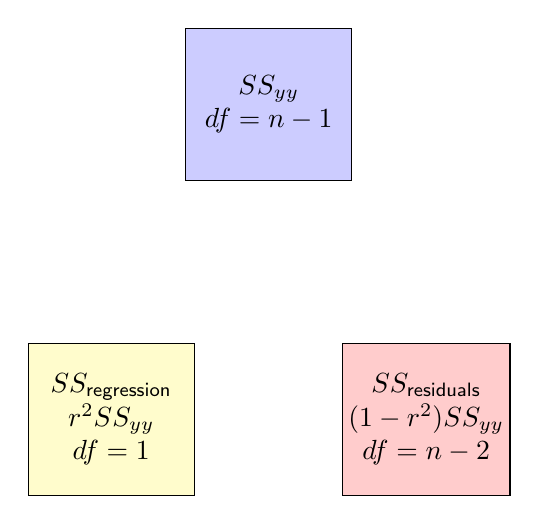
\begin{tikzpicture}
                        \node[draw,fill=blue!20,rectangle,align=center,minimum height=5.5em,
                            minimum width=6em,inner sep=0.5ex,font=\sffamily]
                            at (0,2) {$SS_{yy}$\\ $df = n-1$};
                        \node[draw,fill=yellow!20,rectangle,align=center,minimum height=5.5em,
                            minimum width=6em,inner sep=0.5ex,font=\sffamily]
                            at (-2,-2) {$SS_{\mathsf{regression}}$ \\ $r^2SS_{yy}$ \\$df = 1$};
                        \node[draw,fill=red!20,rectangle,align=center,minimum height=5.5em,
                            minimum width=6em,inner sep=0.5ex,font=\sffamily]
                            at (2,-2) {$SS_{\mathsf{residuals}}$ \\ $(1-r^2)SS_{yy}$ \\$df = n-2$ };
                    \end{tikzpicture}
                }
            \end{figure}
        \end{block}
    \end{columns}
\end{frame}

\begin{frame}
    \frametitle{$\chi^2$ statistic}
    \begin{columns}
        \column{0.5\textwidth}
        \begin{block}{Goodness of fit}
            \begin{itemize}
                \item How good is your model?
                \item observed and expected frequency
                \item $\chi^2$ distribution
            \end{itemize}
            We define the $\chi^2$ as
            \begin{equation}
                \chi^2 = \sum \frac{(f_o-f_e)^2}{f_e}
            \end{equation}
        \end{block}
        \column{0.5\textwidth}
        \begin{block}{}
            \begin{figure}
                \begin{center}
                    \includegraphics[scale=0.06]{img/chi2.png}
                    % http://statwiki.ucdavis.edu/Under_Construction/Chi-Square_Tests_and_F-Tests/11.1_Chi-Square_Tests_for_Independence
                \end{center}
            \end{figure}
        \end{block}
    \end{columns}
\end{frame}

\begin{frame}
    \frametitle{Examples/Discussion}
    \begin{itemize}
        \item Link to examples \url{https://github.com/tbs1980/CISLQuantWorkshop/tree/master/AdvancedQuantitativeMethodsClinic/examples}
        \item Use the rest of the time for examples/discussion.
    \end{itemize}
\end{frame}

\section{Discussion and Summary}

\begin{frame}
    \frametitle{Best practices: let the data speak}
    \begin{table}
        \centering
        \begin{tabular}{|c|c|}
            \hline
            $\times$ & \checkmark \\
            \hline
            majority respondents & 60\% of the respondents \\
            shows large variation & sample variance is \\
            large scatter & no correlation $r=0.001$ \\
            treatment has an impact & the hypothesis tests shows that \\
            cannot be sure & ANOVA shows that \\
            we can confident & the probability oddes from $F$-test was \\
            no difference between methods & $t$-statistic was calculated to be \\
            \hline
        \end{tabular}
    \end{table}
\end{frame}

\begin{frame}
    \frametitle{Summary}
    \begin{itemize}
        \item Descriptive and inferential statistics
        \item Hypotheis testing
        \item Regression
        \item Best practices
    \end{itemize}
\end{frame}

\begin{frame}
    \frametitle{References}
    \begin{itemize}
        \item \alert{Gravetter and Wallnau},\emph{Statistics for the Behavioral Sciences}, 2013
        \item \alert{Wilcox}, \emph{Introduction to Robust Estimation and Hypothesis Testing}, 2012
        \item \alert{Grimmet}, \emph{Probability and Random Processes}, 2001
        \item \alert{Jaynes}, \emph{Probability Theory, The Logic of Science}, 2003
        \item \alert{Sivia and Skilling}, \emph{Data Analysis, A Bayesian Tutorial}, 2006
    \end{itemize}
\end{frame}


\end{document}
